\documentclass[10pt]{article}

\usepackage{amsmath}
%
\usepackage{amssymb}
%
\usepackage{enumerate}
%
\usepackage[width=7in,height=10in,top=0.75in,centering]{geometry}
%
\usepackage[dvipsnames]{xcolor}
%
\usepackage{tikz}
%
\usepackage{multicol}
%
\usepackage{hyperref}
%
\usepackage{marginnote}
%
%%%%%%%%%%%%%%%% HEADER %%%%%%%%%%%%%%%%%%%%%
\usepackage{fancyhdr}
\pagestyle{fancy}
%%
%\lfoot{Left footer}
%\cfoot{Center of footer}
%\rfoot{Right of footer}
%%
\lhead{Survey of Calculus I}
\chead{Week 5 Workshop}
\rhead{\thepage}
%
%%%%%%%%%%%%%%%% HEADER %%%%%%%%%%%%%%%%%%%%%
%
%%%%%%%%%%%%%%%% PGFPLOTS %%%%%%%%%%%%%%%%%%%
\usepackage{pgfplots}
%
\pgfplotsset{every axis/.append style={
                    axis x line=middle,    % put the x axis in the middle
                    axis y line=middle,    % put the y axis in the middle
                    axis line style={<->,color=black}, % arrows on the axis
                    %xlabel={$x$},          % default put x on x-axis
                    ylabel={$y$},          % default put y on y-axis
            }}
%
 \pgfplotsset{compat=1.14}
%
 \usepgfplotslibrary{fillbetween}
%%%%%%%%%%%%%%%% PGFPLOTS %%%%%%%%%%%%%%%%%%%
%
\parindent0pt
\fboxsep=0.25cm
%
\newcommand{\Heading}[2]{\fbox{{\Large\textbf{#1}}}\hfill\fbox{\textbf{#2}}\par\vspace{0.1in}}
%
\newcommand{\Name}[1]{\textbf{Name}:\quad#1\hrulefill}
%
\newcommand{\Target}[1]{\textbf{Learning Target(s):}\quad\fbox{#1}\par\medskip}
%
\DeclareMathOperator{\arcsec}{arcsec}
\DeclareMathOperator{\arccot}{arccot}
\DeclareMathOperator{\arccsc}{arccsc}
%
\newcounter{example}[section]
\newcounter{exercise}[section]
%
\newcommand{\important}[2]{\begin{center}\fbox{\begin{minipage}{.97\textwidth}\noindent\textbf{#1}\par#2\end{minipage}}\end{center}}
%
\newcommand{\defn}[1]{\begin{center}\fbox{\begin{minipage}{.97\textwidth}\reversemarginpar\marginnote{\textbf{Definition}}#1\end{minipage}}\end{center}}
%
\newcommand{\example}[1]{\vspace{0.1in}{\textcolor{blue}{\textbf{Example \stepcounter{example}\theexample.}}}\hspace{0.1in}\reversemarginpar\marginnote{\fbox{\bf #1}}}
%
\newcommand{\exercise}[1]{\vspace{0.1in}{\textcolor{blue}{\textbf{Exercise \stepcounter{exercise}\Alph{exercise}.}}}\hspace{0.1in}\reversemarginpar\marginnote{\fbox{\bf #1}}}

%%%%%%%%%%%% BEGIN DOCUMENT %%%%%%%%%%%%%%%
%%%%%%%%%%%% BEGIN DOCUMENT %%%%%%%%%%%%%%%
%%%%%%%%%%%% BEGIN DOCUMENT %%%%%%%%%%%%%%%
%%%%%%%%%%%% BEGIN DOCUMENT %%%%%%%%%%%%%%%
%%%%%%%%%%%% BEGIN DOCUMENT %%%%%%%%%%%%%%%

\begin{document}

\thispagestyle{empty}

\Heading{MATH 1190 \& 1210 Survey of Calculus I}{\begin{minipage}{0.25\textwidth}\begin{center} Week 5 Workshop \end{center}\end{minipage}}

\vspace{0.1in}

\Name{} \quad \Target{}


Let $p(x)=f(x)g(x)$ and let $q(x)=\dfrac{f(x)}{g(x)}$, where $f$ and $g$ are functions whose graphs are shown below.\\ What are the following values?\\ (a). $p'(-3)$\\ (b). $p'(5)$ \\ (c). $q'(-3)$\\ (d). $q'(5)$



    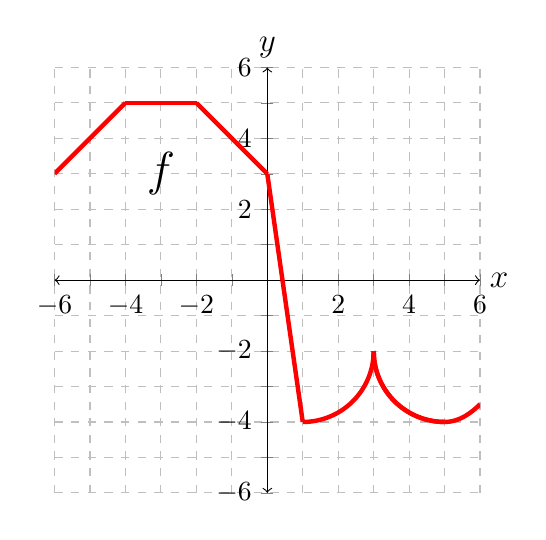
\begin{tikzpicture}[scale=1]
          \begin{axis}[
        %    axis y line = left,
        %    axis x line = bottom,
            xlabel = {\large$x$},
                            xlabel style={anchor=west},
            ylabel = {\large$y$},
                            ylabel style={anchor=south},
            xtick       = {-6,-5, -4, -3,-2,-1,1,2,3, 4, 5, 6},
            xticklabels = {$-6$, , $-4$, ,$-2$,,,$2$,, $4$, , $6$},
            ytick       = {-6,-5, -4, -3,-2,-1,1,2,3, 4, 5, 6},
            yticklabels = {$-6$, , $-4$, ,$-2$,,,$2$,, $4$, , $6$},
            samples     = 160,
            domain      = 0:3,
            restrict y to domain=-10:100,
            xmin = -6, xmax = 6,
            ymin = -6, ymax = 6,
            width=2.75in,height=2.75in,
            grid=both, grid style=dashed
          ]
          %
          \addplot[domain=-6:-4, red, ultra thick, mark=none] {x + 9};
          %
          \addplot[domain=-4:-2, red, ultra thick, mark=none] {5};
          %
          \addplot[domain=-2:0, red, ultra thick, mark=none] {-x + 3};
          %
          \addplot[domain=0:1, red, ultra thick, mark=none] {-7*x+3};
          \addplot[domain=1:3, red, ultra thick, mark=none] {-2 - (4 - (x-1)^2)^(0.5)};
          \addplot[domain=3:5, red, ultra thick, mark=none] {-2 - (4 - (x-5)^2)^(0.5)};
          \addplot[domain=3:5, red, ultra thick, mark=none] {-2 - (4 - (x-5)^2)^(0.5)};
          \addplot[domain=5:6, red, ultra thick, mark=none] {-4 + 0.5*(x-5)^2};
          %
          \filldraw[black] (-3,3) circle (0pt) node[] {\LARGE $f$};



         
        \end{axis}
    \end{tikzpicture}    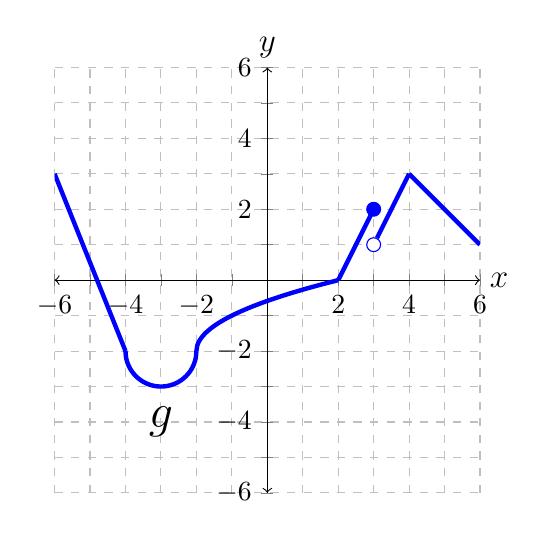
\begin{tikzpicture}[scale=1]
          \begin{axis}[
        %    axis y line = left,
        %    axis x line = bottom,
            xlabel = {\large$x$},
                            xlabel style={anchor=west},
            ylabel = {\large$y$},
                            ylabel style={anchor=south},
            xtick       = {-6,-5, -4, -3,-2,-1,1,2,3, 4, 5, 6},
            xticklabels = {$-6$, , $-4$, ,$-2$,,,$2$,, $4$, , $6$},
            ytick       = {-6,-5, -4, -3,-2,-1,1,2,3, 4, 5, 6},
            yticklabels = {$-6$, , $-4$, ,$-2$,,,$2$,, $4$, , $6$},
            samples     = 160,
            domain      = 0:3,
            restrict y to domain=-10:100,
            xmin = -6, xmax = 6,
            ymin = -6, ymax = 6,
            width=2.75in,height=2.75in,
            grid=both, grid style=dashed
          ]
          %
%          \addplot[domain=-6:-4, red, ultra thick, mark=none] {x + 9};
%          %
%          \addplot[domain=-4:-3, red, ultra thick, mark=none] {5};
%          %
%          \addplot[domain=-3:0, red, ultra thick, mark=none] {-2/3 * x + 3};
%          %
%          \addplot[domain=0:1, red, ultra thick, mark=none] {-7*x+3};
%          \addplot[domain=1:3, red, ultra thick, mark=none] {-2 - (4 - (x-1)^2)^(0.5)};
%          \addplot[domain=3:5, red, ultra thick, mark=none] {-2 - (4 - (x-5)^2)^(0.5)};
%          \addplot[domain=3:5, red, ultra thick, mark=none] {-2 - (4 - (x-5)^2)^(0.5)};
%          \addplot[domain=5:6, red, ultra thick, mark=none] {-4 + 0.5*(x-5)^2};
%          %
%          \filldraw[black] (-3,3) circle (0pt) node[] {\LARGE $f$};
          %
          %\draw[->,thick] (-0.9,1.9) -- (-0.35,1.6);
          %
          \addplot[domain=-6:-4, blue, ultra thick, mark=none] {-5/2 *x -12};
          %
          \addplot[domain=-4:-2, blue, ultra thick, mark=none] {-2 - (1 - (x+3)^2)^(1/2)};
          \addplot[domain=-2:2, blue, ultra thick, mark=none] {(x+2)^(1/2) - 2};
          %
          \addplot[domain=2:3, blue, ultra thick, mark=none] {2*x-4};
          \addplot[domain=3:4, blue, ultra thick, mark=none] {2*x-5};
          \filldraw[white] (3,1) circle (2.5pt);
          \draw[blue] (3,1) circle (2.5pt);
          \filldraw[blue] (3,2) circle (2.5pt);
          \addplot[domain=4:6, blue, ultra thick, mark=none] {-x+7};
          %
          \filldraw[black] (-3,-4) circle (0pt) node[] {\LARGE $g$};
          %
          %\draw[->,thick] (0.3,-1.5) -- (-0.2,-1.3);
          %
        \end{axis}
    \end{tikzpicture}    

\vfill

Let $k(x)=f(g(x))$, where $f$ and $g$ are functions whose graphs are shown below. \\ What are the following values?\\ (a). $k'(-3)$\\ (b). $k'(5)$



    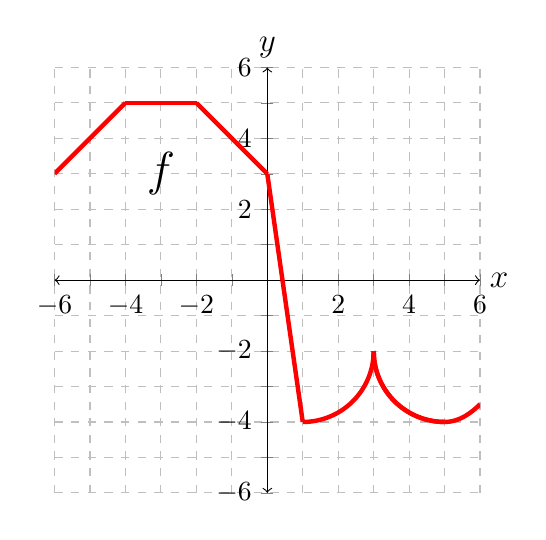
\begin{tikzpicture}[scale=1]
          \begin{axis}[
        %    axis y line = left,
        %    axis x line = bottom,
            xlabel = {\large$x$},
                            xlabel style={anchor=west},
            ylabel = {\large$y$},
                            ylabel style={anchor=south},
            xtick       = {-6,-5, -4, -3,-2,-1,1,2,3, 4, 5, 6},
            xticklabels = {$-6$, , $-4$, ,$-2$,,,$2$,, $4$, , $6$},
            ytick       = {-6,-5, -4, -3,-2,-1,1,2,3, 4, 5, 6},
            yticklabels = {$-6$, , $-4$, ,$-2$,,,$2$,, $4$, , $6$},
            samples     = 160,
            domain      = 0:3,
            restrict y to domain=-10:100,
            xmin = -6, xmax = 6,
            ymin = -6, ymax = 6,
            width=2.75in,height=2.75in,
            grid=both, grid style=dashed
          ]
          %
          \addplot[domain=-6:-4, red, ultra thick, mark=none] {x + 9};
          %
          \addplot[domain=-4:-2, red, ultra thick, mark=none] {5};
          %
          \addplot[domain=-2:0, red, ultra thick, mark=none] {-x + 3};
          %
          \addplot[domain=0:1, red, ultra thick, mark=none] {-7*x+3};
          \addplot[domain=1:3, red, ultra thick, mark=none] {-2 - (4 - (x-1)^2)^(0.5)};
          \addplot[domain=3:5, red, ultra thick, mark=none] {-2 - (4 - (x-5)^2)^(0.5)};
          \addplot[domain=3:5, red, ultra thick, mark=none] {-2 - (4 - (x-5)^2)^(0.5)};
          \addplot[domain=5:6, red, ultra thick, mark=none] {-4 + 0.5*(x-5)^2};
          %
          \filldraw[black] (-3,3) circle (0pt) node[] {\LARGE $f$};



         
        \end{axis}
    \end{tikzpicture}    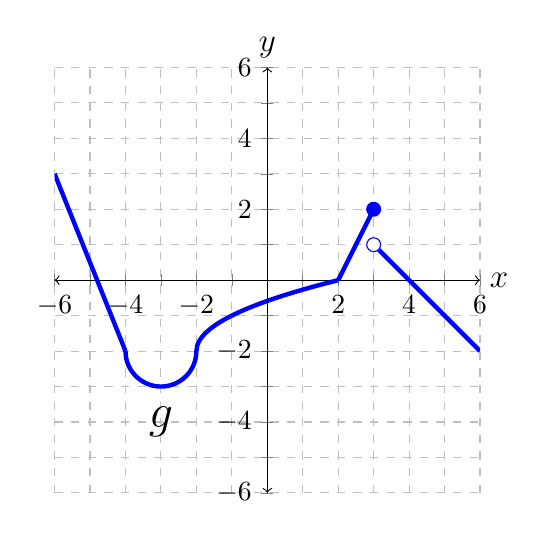
\begin{tikzpicture}[scale=1]
          \begin{axis}[
        %    axis y line = left,
        %    axis x line = bottom,
            xlabel = {\large$x$},
                            xlabel style={anchor=west},
            ylabel = {\large$y$},
                            ylabel style={anchor=south},
            xtick       = {-6,-5, -4, -3,-2,-1,1,2,3, 4, 5, 6},
            xticklabels = {$-6$, , $-4$, ,$-2$,,,$2$,, $4$, , $6$},
            ytick       = {-6,-5, -4, -3,-2,-1,1,2,3, 4, 5, 6},
            yticklabels = {$-6$, , $-4$, ,$-2$,,,$2$,, $4$, , $6$},
            samples     = 160,
            domain      = 0:3,
            restrict y to domain=-10:100,
            xmin = -6, xmax = 6,
            ymin = -6, ymax = 6,
            width=2.75in,height=2.75in,
            grid=both, grid style=dashed
          ]
          %
%          \addplot[domain=-6:-4, red, ultra thick, mark=none] {x + 9};
%          %
%          \addplot[domain=-4:-3, red, ultra thick, mark=none] {5};
%          %
%          \addplot[domain=-3:0, red, ultra thick, mark=none] {-2/3 * x + 3};
%          %
%          \addplot[domain=0:1, red, ultra thick, mark=none] {-7*x+3};
%          \addplot[domain=1:3, red, ultra thick, mark=none] {-2 - (4 - (x-1)^2)^(0.5)};
%          \addplot[domain=3:5, red, ultra thick, mark=none] {-2 - (4 - (x-5)^2)^(0.5)};
%          \addplot[domain=3:5, red, ultra thick, mark=none] {-2 - (4 - (x-5)^2)^(0.5)};
%          \addplot[domain=5:6, red, ultra thick, mark=none] {-4 + 0.5*(x-5)^2};
%          %
%          \filldraw[black] (-3,3) circle (0pt) node[] {\LARGE $f$};
          %
          %\draw[->,thick] (-0.9,1.9) -- (-0.35,1.6);
          %
          \addplot[domain=-6:-4, blue, ultra thick, mark=none] {-5/2 *x -12};
          %
          \addplot[domain=-4:-2, blue, ultra thick, mark=none] {-2 - (1 - (x+3)^2)^(1/2)};
          \addplot[domain=-2:2, blue, ultra thick, mark=none] {(x+2)^(1/2) - 2};
          %
          \addplot[domain=2:3, blue, ultra thick, mark=none] {2*x-4};
          \addplot[domain=3:4, blue, ultra thick, mark=none] {-x+4};
          \filldraw[white] (3,1) circle (2.5pt);
          \draw[blue] (3,1) circle (2.5pt);
          \filldraw[blue] (3,2) circle (2.5pt);
          \addplot[domain=4:6, blue, ultra thick, mark=none] {-x+4};
          %
          \filldraw[black] (-3,-4) circle (0pt) node[] {\LARGE $g$};
          %
          %\draw[->,thick] (0.3,-1.5) -- (-0.2,-1.3);
          %
        \end{axis}
    \end{tikzpicture}

Let $f(x)$ and $g(x)$ be functions with the following values:$$
\begin{array}{|c|c|c|c|c|}
\hline
x & f(x) & f'(x) & g(x) & g'(x) \\
\hline
0 & 0 & -1 & 2 & 1/2 \\
1 & 1 & -2 & 0 & 0\\
\hline
\end{array}
$$
Compute the following derivatives. Try to identify the outermost functions, then break them down to find each derivative separately.
\begin{enumerate}[(a)]
    \item $$\frac{d}{dx} \left[ \frac{ (f(1-x))^2 }{ x^3 + 1 } \right]_{x=1}.$$
    \item $$\frac{d}{dx} \left[ f(x^2 - 1) \cdot g(2x - 1) \right]_{x=1}.$$
    \item $$\frac{d}{dx} \left[ \frac{f(x^2-2x+1)}{\sqrt{g(x) + 5}} \right]_{x=1}.$$
\end{enumerate}
\end{document}
